\documentclass[xcolor=dvipsnames]{beamer}
\usepackage[T1]{fontenc}
\usepackage[utf8]{inputenc}
\usepackage[english,slovak]{babel}

\usepackage{amsmath}
\usepackage{amsthm}
\usetheme{Pittsburgh}
\useoutertheme{shadow}

\usepackage{graphicx}
\usepackage{caption}
\usepackage{subcaption}

\usepackage[]{algorithm2e}
\usepackage{listings}
 \setbeamercovered{transparent}
 \usepackage{cuted}
\usepackage[export]{adjustbox}
\usepackage{mathtools}

\usepackage{lipsum}
\usepackage{verbatim}
\usepackage{transparent}
\usepackage{framed}
\usepackage{xcolor}

\usepackage{multirow}
\usepackage{colortbl}
\usepackage{lmodern}

\usepackage{hyperref}

\usepackage{movie15}


\iftrue

\usetheme{Warsaw}

\setbeamercolor{normal text}{fg=white,bg=black!90}
\setbeamercolor{structure}{fg=white}

\setbeamercolor{alerted text}{fg=red!85!black}

\setbeamercolor{item projected}{use=item,fg=black,bg=item.fg!35}

\setbeamercolor*{palette primary}{use=structure,fg=structure.fg}
\setbeamercolor*{palette secondary}{use=structure,fg=structure.fg!95!black}
\setbeamercolor*{palette tertiary}{use=structure,fg=structure.fg!90!black}
\setbeamercolor*{palette quaternary}{use=structure,fg=structure.fg!95!black,bg=black!80}

\setbeamercolor*{framesubtitle}{fg=white}

\setbeamercolor*{block title}{parent=structure,bg=black!60}
\setbeamercolor*{block body}{fg=black,bg=black!10}
\setbeamercolor*{block title alerted}{parent=alerted text,bg=black!15}
\setbeamercolor*{block title example}{parent=example text,bg=black!15}

\fi



%-------------------------------------------------------------------------------------
\title{\color{white} \bf Reinforcement learning experiments}
\author{\color{white} Michal CHOVANEC, PhD}


%\setbeamertemplate{footline}[frame number]{}
\setbeamertemplate{navigation symbols}{}


\date[EURP]{}
\begin{document}

{
    \usebackgroundtemplate
    {
        \vbox to \paperheight{\vfil\hbox to \paperwidth{\hfil

        {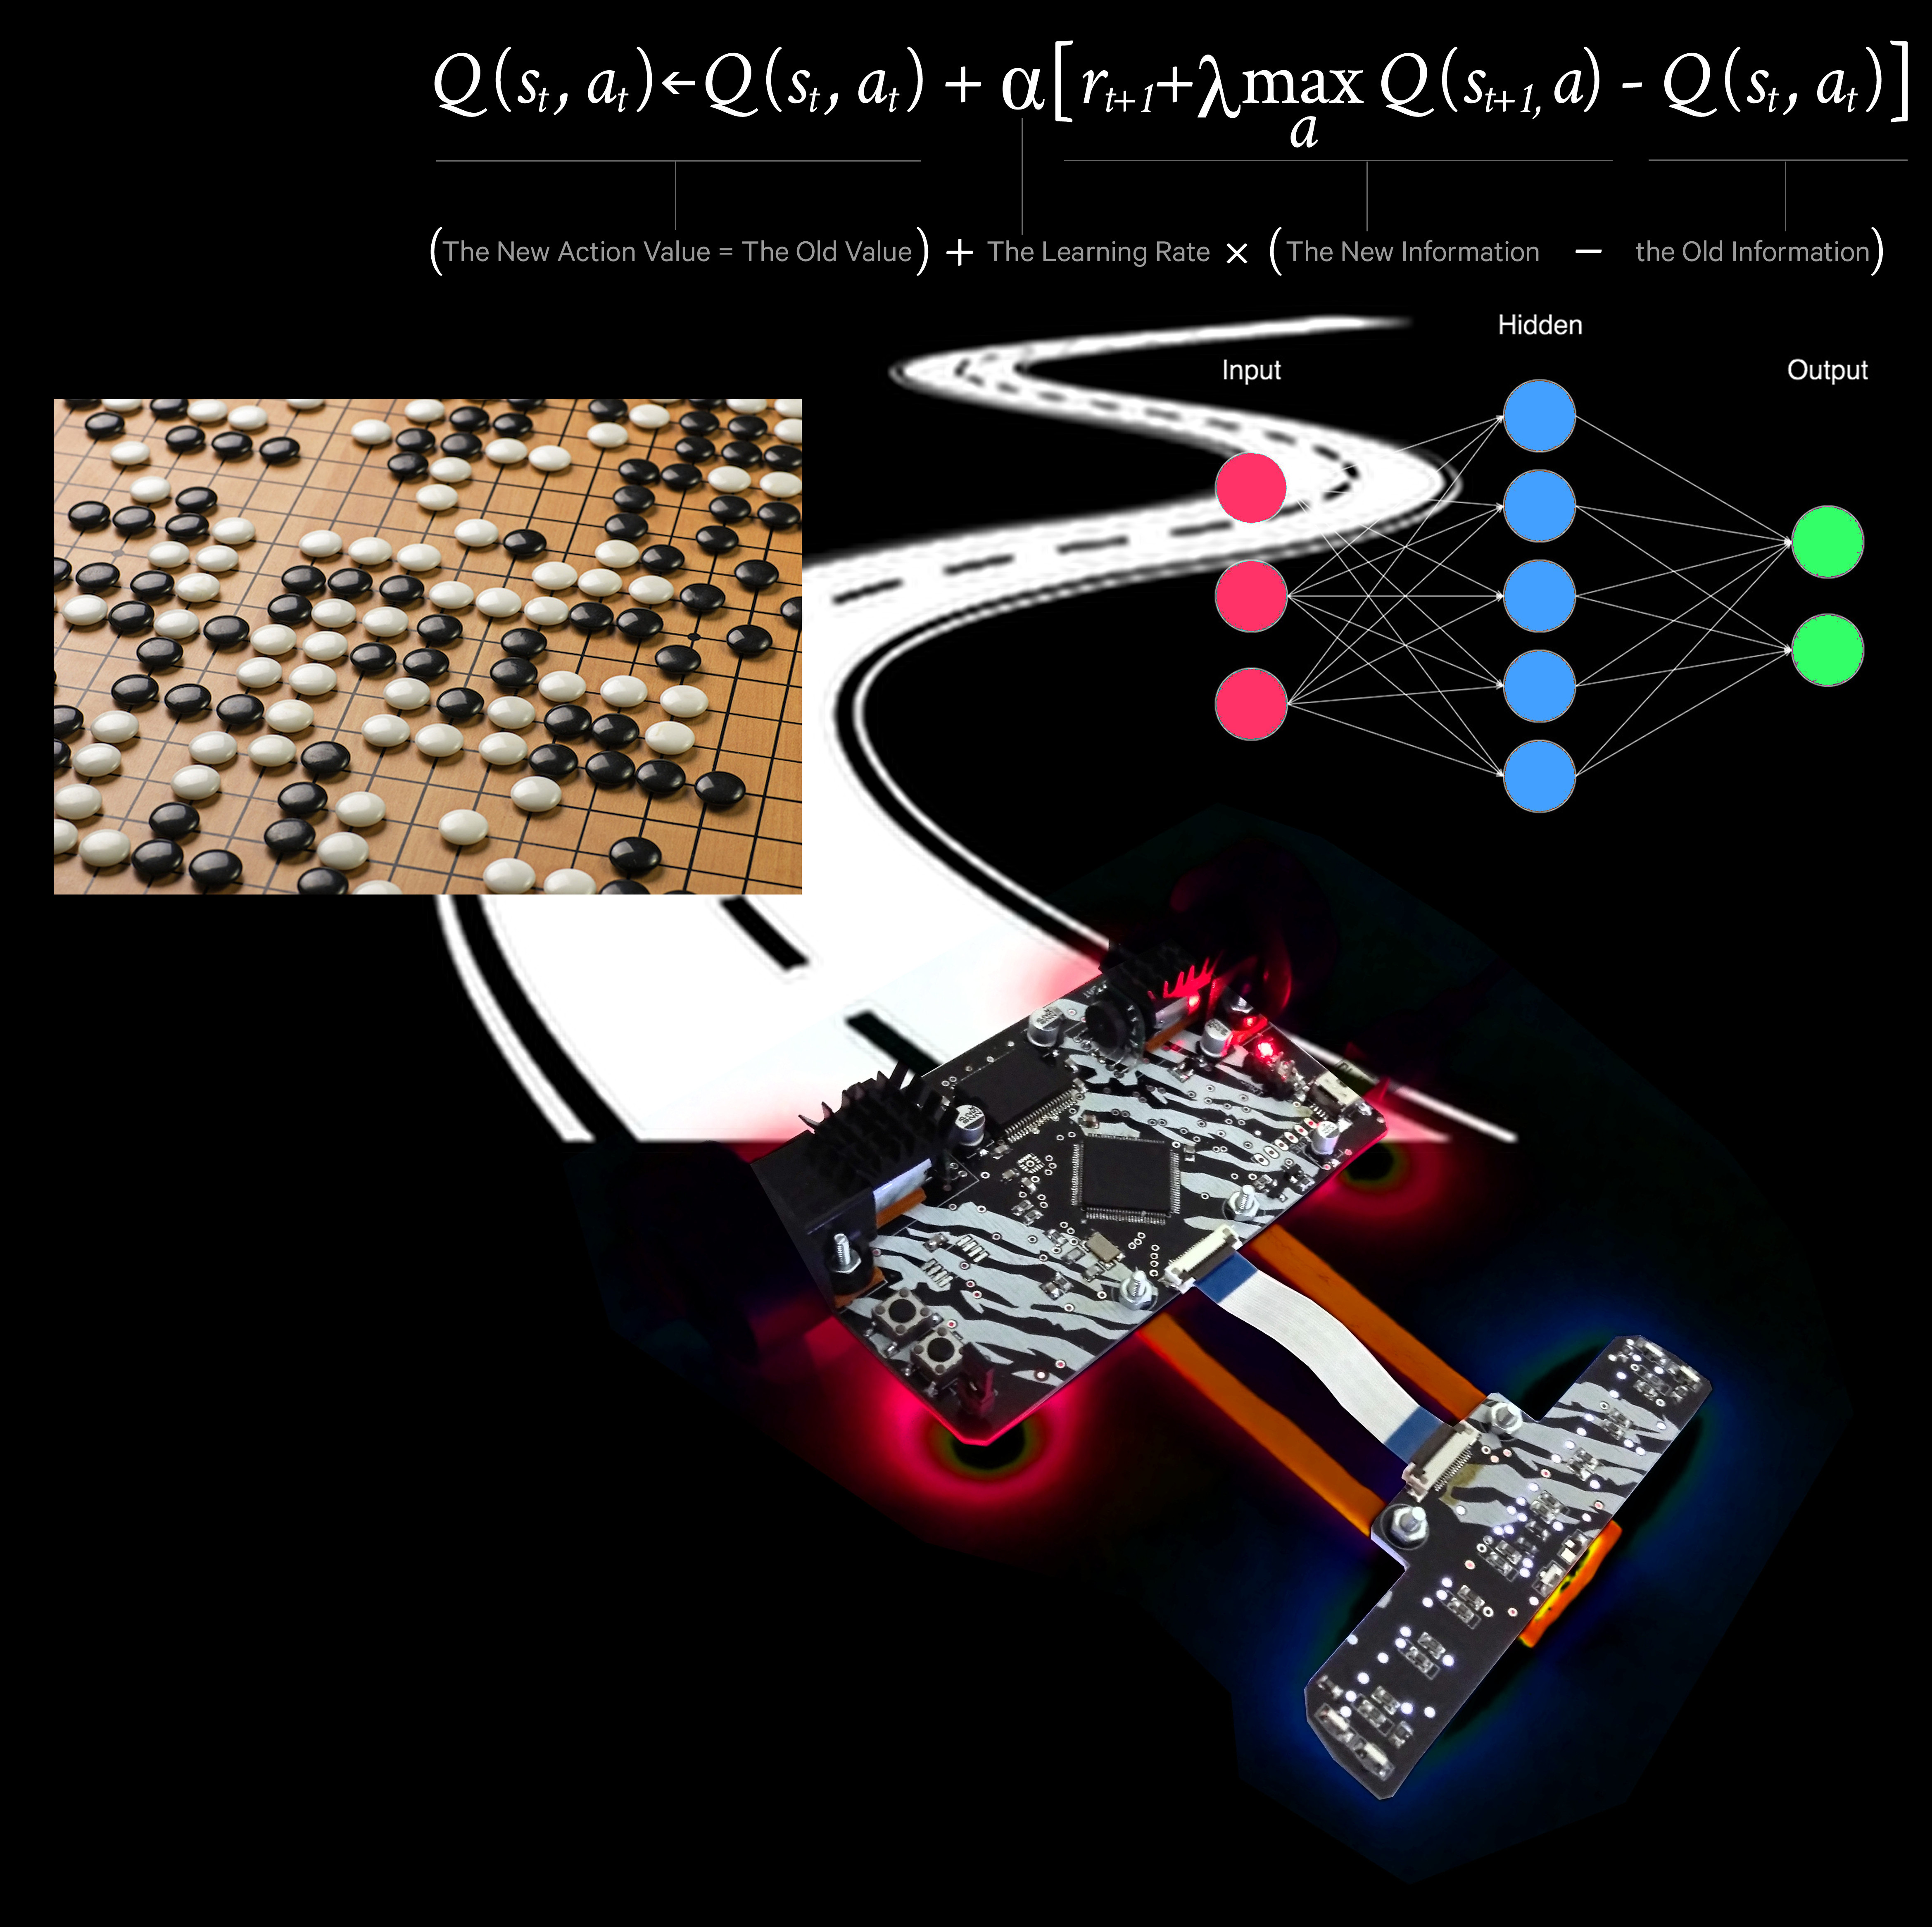
\includegraphics[width=5.05in]{../../pictures/rl_square.jpg}}

        \hfil}\vfil}
    }
    \begin{frame}

    %\titlepage


    \centering
     \colorbox{black}
     {
        \begin{minipage}{7cm}
           {\LARGE \color{white} \bf Reinforcement learning experiments} \\
           {\LARGE \color{white} Michal CHOVANEC, PhD} \\
       \end{minipage}
     }


    \end{frame}
}

\begin{frame}{\bf Reinforcement learning}

\begin{columns}
\begin{column}{0.5\textwidth}

    \begin{itemize}
      \item obtain {\bf state}
      \item choose {\bf action}
      \item {\bf execute} action
      \item obtain {\bf reward}
      \item learn from {\bf experiences}
      \item function {\bf $Q(s, a)$}, how good is action $a$ in state $s$
    \end{itemize}

      \begin{figure}
        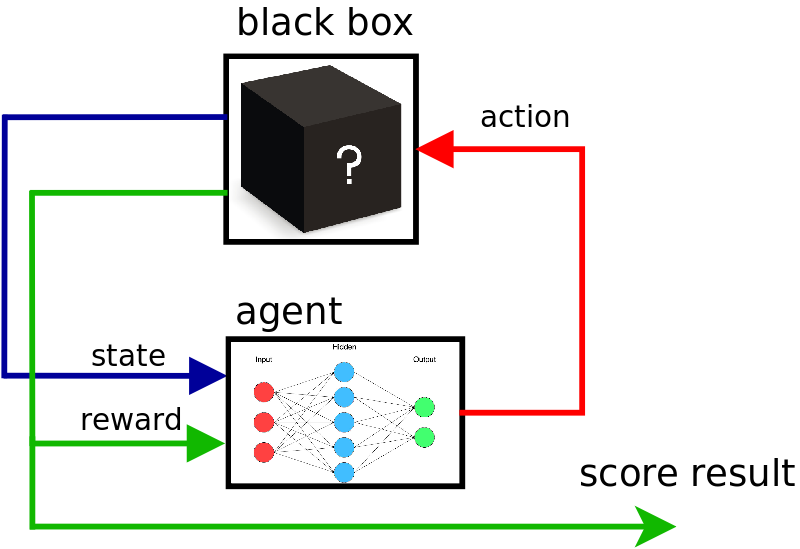
\includegraphics[scale=0.2]{../../diagrams/rl_mechanism.png}
      \end{figure}

\end{column}
\begin{column}{0.5\textwidth}  %%<--- here

      \begin{itemize}
      \item {\bf playing Atari}
      \item {\bf playing Doom}
      \item {\bf playing GO}
    \end{itemize}


    \begin{figure}[!htb]
      \centering
      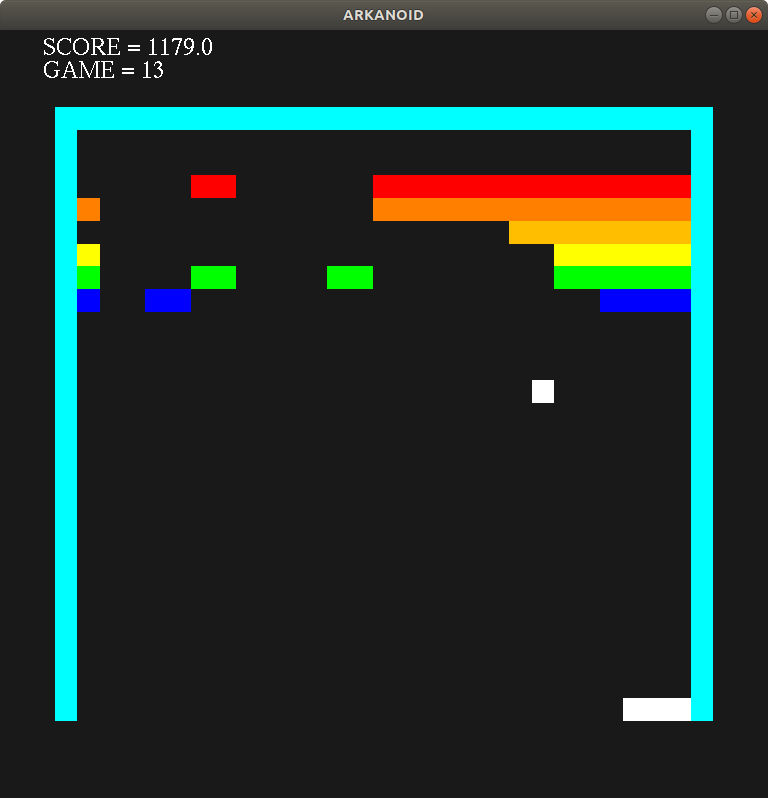
\includegraphics[scale=0.15]{../../diagrams/rl/arkanoid.png}
    \end{figure}

\end{column}
\end{columns}

\end{frame}

\begin{frame}{\bf Deep Q network}

{
    \footnotesize
    \begin{itemize}
    \item {\bf \color{red} correlated states} : experience replay buffer
    \item {\bf \color{red} unstable training} : non-stationary target value $\hat{Q}(s, a; w)$, depends on $w$, use temporary fixed weights w'
    \item {\bf \color{red} unknow gradients values} : clip or normalise rewards, Q values and gradients into $\langle -1, 1 \rangle$
    \end{itemize}
}
\begin{align*}
  \hat{Q}(s, a; w) &= R + \gamma \max \limits_{\alpha'} \hat{Q}(s', \alpha'; w') \\
  \mathcal{L} &= ( R + \gamma \max \limits_{\alpha'} \hat{Q}(s', \alpha'; w') - \hat{Q}(s, a; w) )^2
  \label{eq:dqn}
\end{align*}
\begin{figure}[!htb]
  \centering
  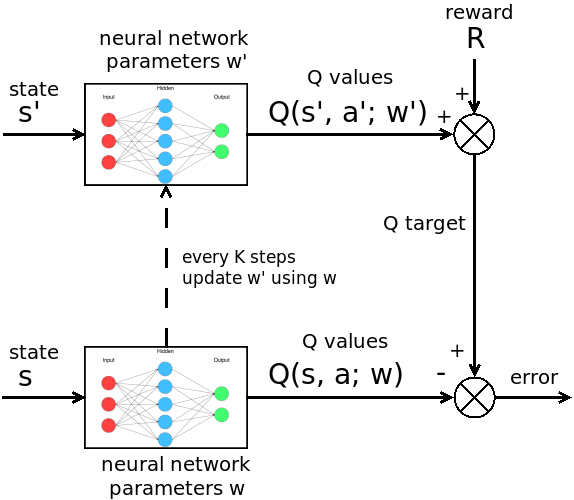
\includegraphics[scale=0.16]{../../diagrams/dqn.png}
  \label{img:dqn}
\end{figure}

\end{frame}


\begin{frame}{\bf Networks architecture}

Following modern {\bf State of the art} networks :\\ 3x3 convolutions, 2x2 pooling, ELU activation

{\footnotesize
    \begin{itemize}
        \item Atari
            \begin{itemize}
                \item input : 48x48x12 (rgb x 4 last frames)
                \item network : C3x3x32 - P2x2 - C3x3x32 - P2x2 - C3x3x32 - P2x2 - C3x3x32 - P2x2 - FC256 - FC$_{actions\_count}$
            \end{itemize}
            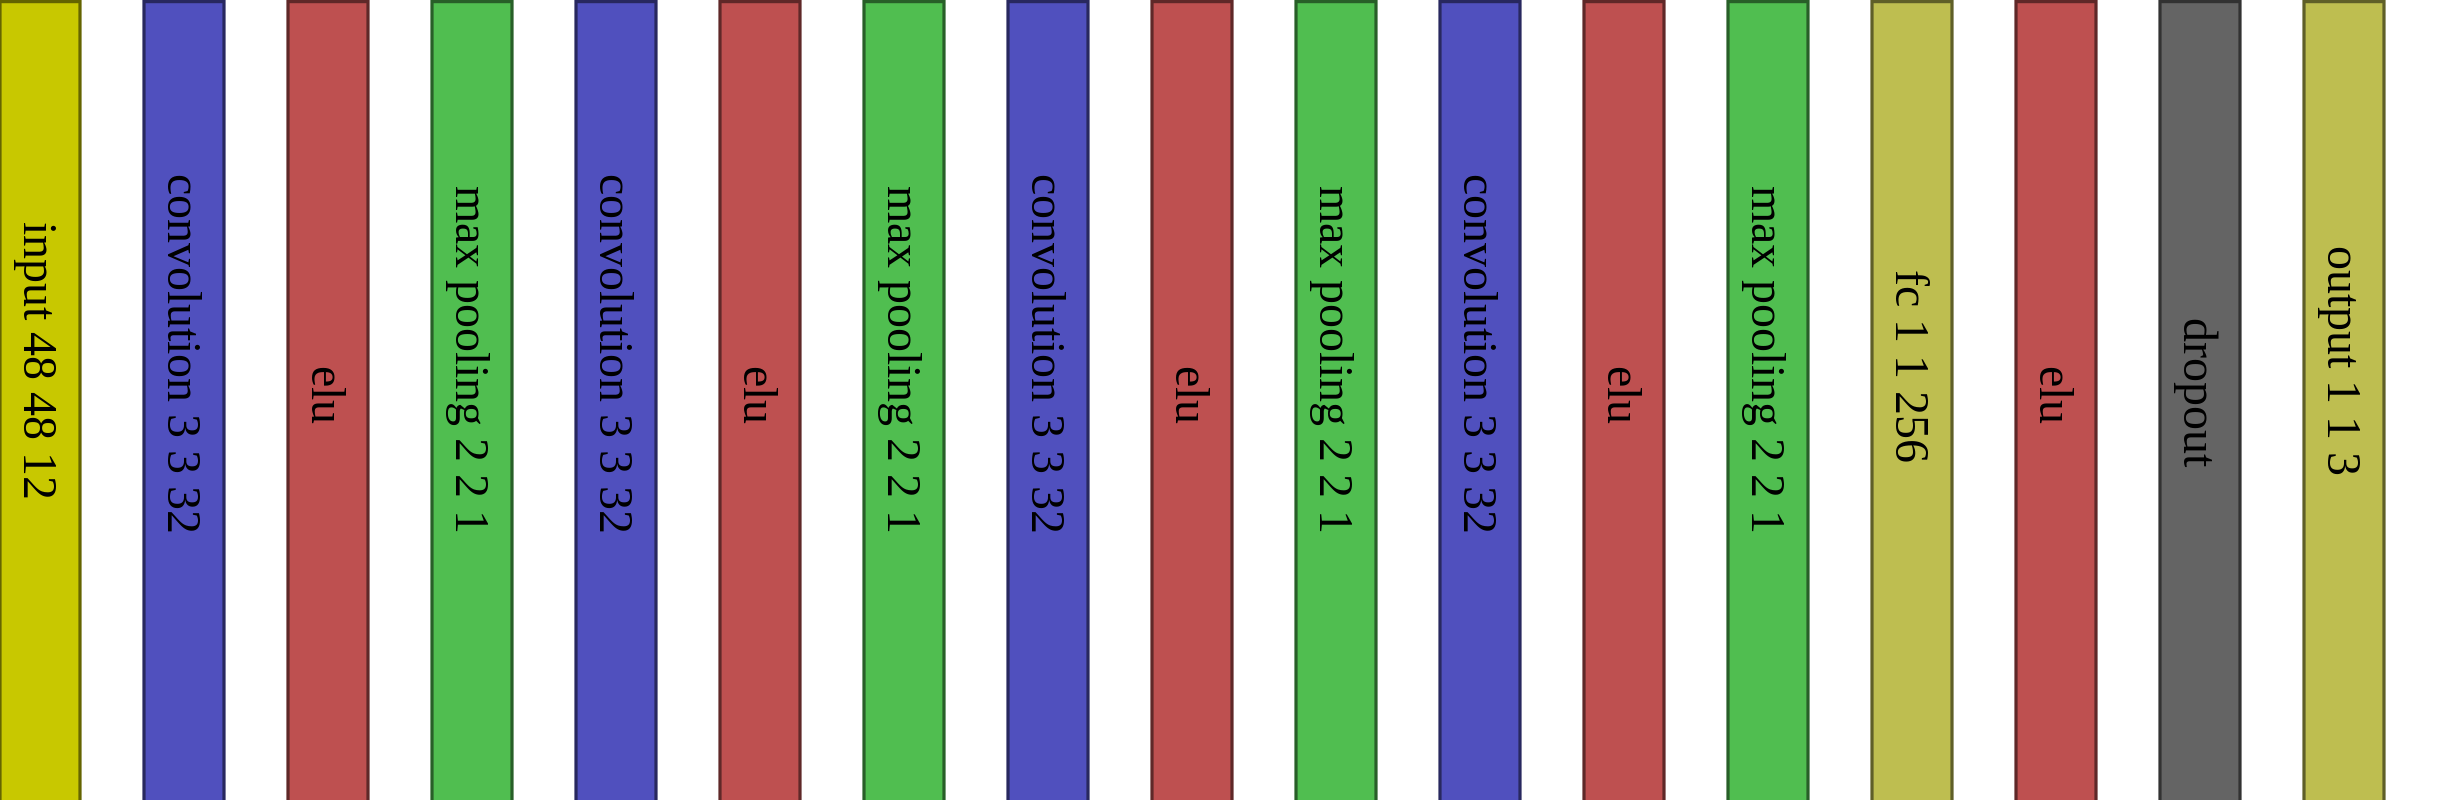
\includegraphics[scale=0.05]{../../diagrams/rl/atari_network.png}

        \item DOOM
            \begin{itemize}
                \item input : 80x80x24 (rgb x 8 last frames)
                \item network : C3x3x64 - P2x2 - C3x3x64 - P2x2 - C3x3x64 - P2x2 - C3x3x64 - P2x2 - FC256 - FC$_{actions\_count}$
            \end{itemize}
            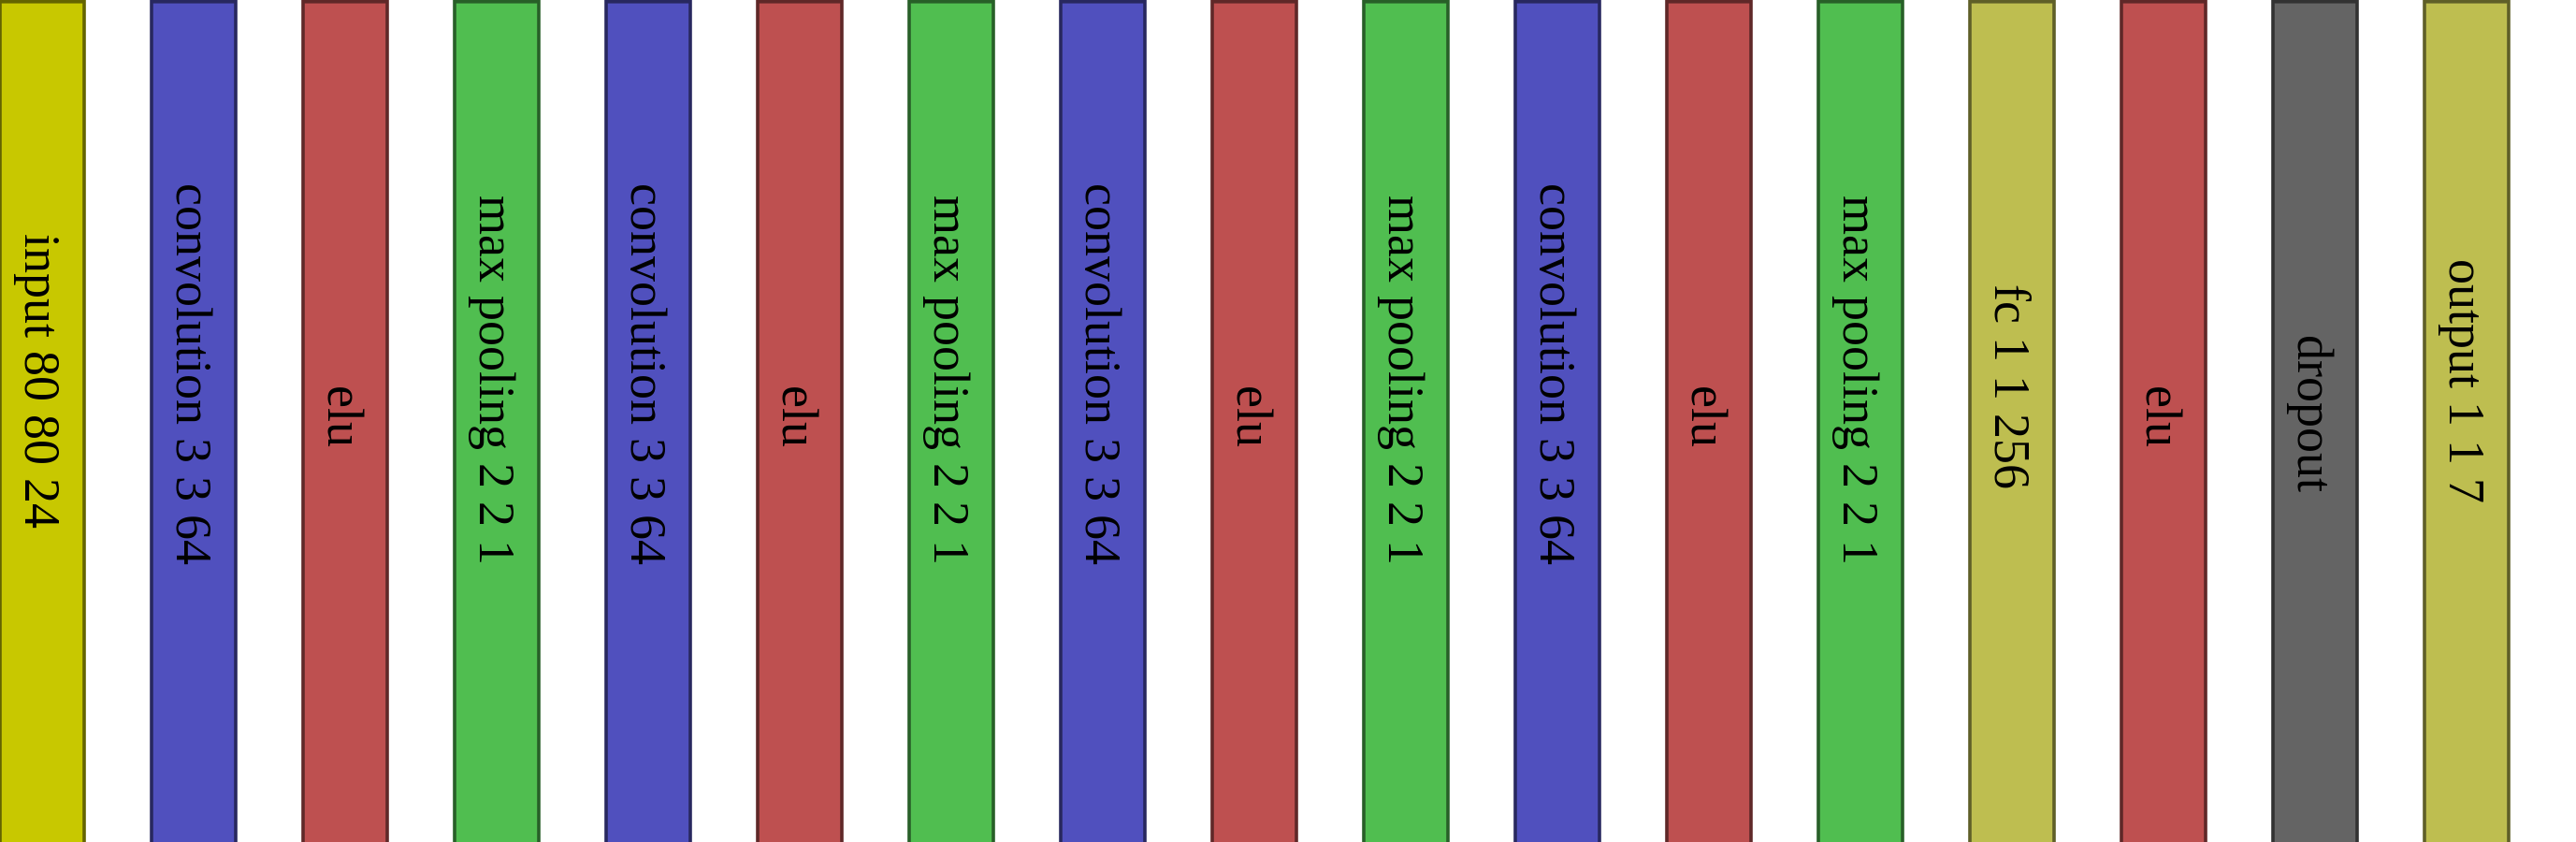
\includegraphics[scale=0.05]{../../diagrams/rl/doom_network.png}

    \end{itemize}
}

\end{frame}


\begin{frame}{\bf GO Network architecture}
we need to go much deeper for GO
\begin{itemize}
  \item {\bf 28, 35 layers} \\ dense blocks + feature pooling layer
  \item {\bf input} \\ 4 matrices $19x19$: black stones, white stones, empty fields, active player
  \item {\bf output} \\ recommended moves 19x19 + 1 for pass = 362 outputs

\end{itemize}

  \begin{figure}[!htb]
    \centering
    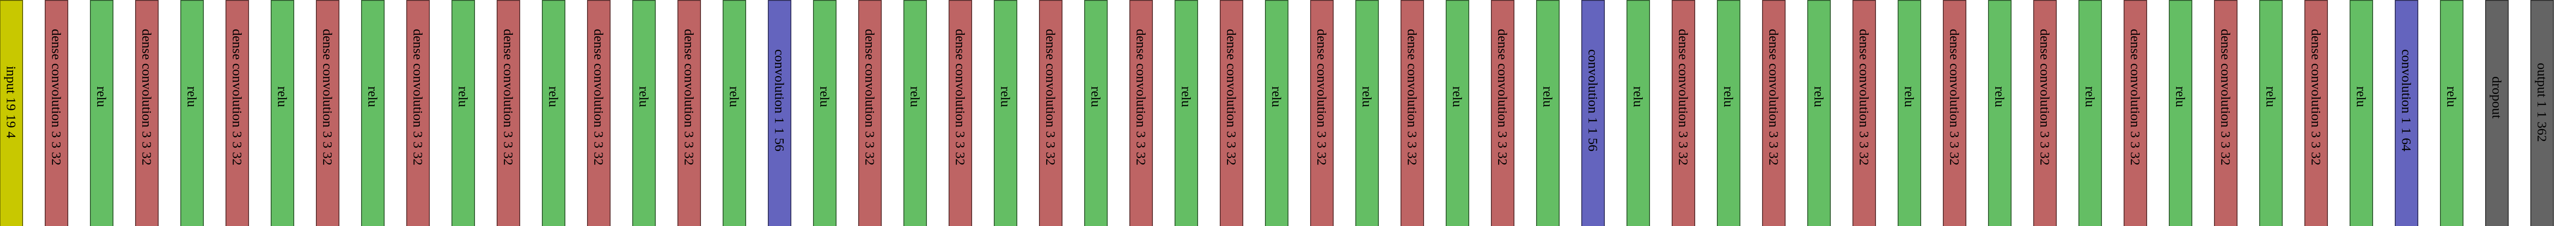
\includegraphics[scale=0.06]{../../diagrams/net_go_1_28_layers.png}
  \end{figure}

  \begin{figure}[!htb]
    \centering
    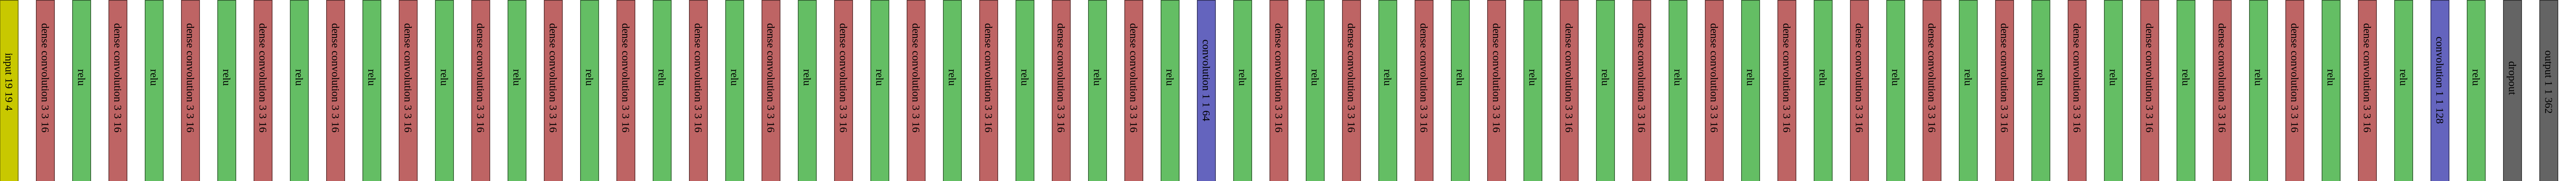
\includegraphics[scale=0.06]{../../diagrams/net_go_5_35_layers.png}
  \end{figure}

\end{frame}

\begin{frame}
All programmed from scratch in C++, Cuda and Python \\ - about 40 000 lines of code :
\begin{itemize}
    \item Rysy CNN framework : \url{https://github.com/michalnand/rysy}
    \item RL framework :  \url{https://github.com/michalnand/rl_examples}
\end{itemize}

\begin{figure}
  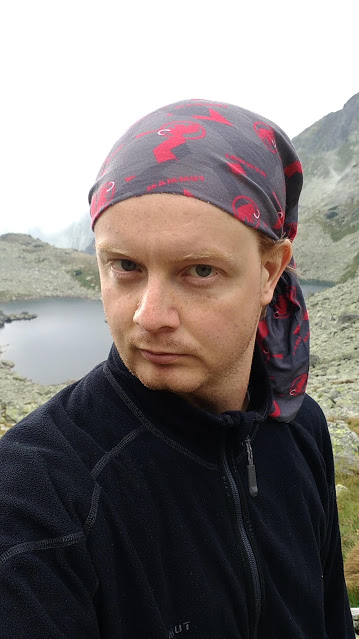
\includegraphics[scale=0.15]{../../pictures/me.jpg}
\end{figure}

\centering {
michal chovanec (michal.nand@gmail.com)
\url{www.youtube.com/channel/UCzVvP2ou8v3afNiVrPAHQGg}
}



\end{frame}


\end{document}
